\documentclass[
	12pt,
	a4paper,
	bibtotoc,
	cleardoubleempty, 
	idxtotoc,
	ngerman,
	openright
	final,
	listof=nochaptergap,
	]{scrbook}

\usepackage[T1]{fontenc}
\usepackage[utf8]{inputenc}

% ##################################################
% Unterstuetzung fuer die deutsche Sprache
% ##################################################
\usepackage{ngerman}
\usepackage[ngerman]{babel}

% ##################################################
% Dokumentvariablen
% ##################################################

% Persoenliche Daten
\newcommand{\docNachnameA}{Grituc}
\newcommand{\docVornameA}{Eugeniu}
\newcommand{\docEmailA}{eugeniu.grituc@hs-furtwangen.de}
\newcommand{\docMatrikelnummerA}{250301}
\newcommand{\docNachnameB}{Halilaj}
\newcommand{\docVornameB}{Ilirian}
\newcommand{\docEmailB}{ilirian.halilaj@hs-furtwangen.de}
\newcommand{\docMatrikelnummerB}{248389}
\newcommand{\docNachnameC}{Oberhauser}
\newcommand{\docVornameC}{Jurek}
\newcommand{\docEmailC}{jurek.oberhauser@hs-furtwangen.de}
\newcommand{\docMatrikelnummerC}{----}
\newcommand{\docNachnameD}{Lang}
\newcommand{\docVornameD}{Maximilian}
\newcommand{\docEmailD}{m.lang@hs-furtwangen.de}
\newcommand{\docMatrikelnummerD}{205853}
\newcommand{\docNachnameE}{Kotzjan}
\newcommand{\docVornameE}{Michael}
\newcommand{\docEmailE}{michael.kotzjan@hs-furtwangen.de}
\newcommand{\docMatrikelnummerE}{250855}

% Dokumentdaten
\newcommand{\docTitle}{FHFTrain}
%\newcommand{\docUntertitle}{} % Kein Untertitel
\newcommand{\docUntertitle}{Simulation eines Zugbetriebes mit Bahnhöfen}
% Arten der Arbeit: Bachelorthesis, Masterthesis, Seminararbeit, Diplomarbeit
\newcommand{\docArtDerArbeit}{Semesterprojekt}
%Studiengaenge: Allgemeine Informatik Bachelor, Computer Networking Bachelor,
% Software-Produktmanagement Bachelor, Advanced Computer Scinece Master
\newcommand{\docStudiengang}{Allgemeine Informatik}
\newcommand{\docAbgabedatum}{----}
\newcommand{\docErsterReferent}{Prof. Dr. Rainer Müller}

% ##################################################
% Allgemeine Pakete
% ##################################################

% Abbildungen einbinden
\usepackage{graphicx}

% Zusaetsliche Sonderzeichen
\usepackage{dingbat}

% Farben
\usepackage{color}
\usepackage[usenames,dvipsnames,svgnames,table]{xcolor}

% Maskierung von URLs und Dateipfaden
\usepackage[hyphens]{url}

% Deutsche Anfuehrungszeichen
\usepackage[babel, german=quotes]{csquotes}

% Pakte zur Index-Erstellung (Schlagwortverzeichnis)
\usepackage{index}
\makeindex

% Ipsum Lorem
% Paket wird nur für das Beispiel gebraucht und kann gelöscht werden
\usepackage{lipsum}

% ##################################################
% Seitenformatierung
% ##################################################
\usepackage[
	portrait,
	bindingoffset=1.5cm,
	inner=2.5cm,
	outer=2.5cm,
	top=3cm,
	bottom=2cm,
	%includeheadfoot
	]{geometry}

% ##################################################
% Kopf- und Fusszeile
% ##################################################

\usepackage{fancyhdr}

\pagestyle{fancy}
\fancyhf{}
\fancyhead[EL,OR]{\sffamily\thepage}
\fancyhead[ER,OL]{\sffamily\leftmark}

\fancypagestyle{headings}{}

\fancypagestyle{plain}{}

\fancypagestyle{empty}{
  \fancyhf{}
  \renewcommand{\headrulewidth}{0pt}
}

%Kein "Kapitel # NAME" in der Kopfzeile
\renewcommand{\chaptermark}[1]{
	\markboth{#1}{}
   	\markboth{\thechapter.\ #1}{}
}

% ##################################################
% Schriften
% ##################################################

% Stdandardschrift festlegen
\renewcommand{\familydefault}{\sfdefault}

% Standard Zeilenabstand: 1,5 zeilig
\usepackage{setspace}
\onehalfspacing 

% Schriftgroessen festlegen
\addtokomafont{chapter}{\sffamily\large\bfseries} 
\addtokomafont{section}{\sffamily\normalsize\bfseries} 
\addtokomafont{subsection}{\sffamily\normalsize\mdseries} 
\addtokomafont{caption}{\sffamily\normalsize\mdseries} 

% ##################################################
% Inhaltsverzeichnis / Allgemeine Verzeichniseinstellungen
% ##################################################

\usepackage{tocloft}

% Punkte auch bei Kapiteln
\renewcommand{\cftchapdotsep}{3}
\renewcommand{\cftdotsep}{3}

% Schriftart und -groesse im Inhaltsverzeichnis anpassen
\renewcommand{\cftchapfont}{\sffamily\normalsize}
\renewcommand{\cftsecfont}{\sffamily\normalsize}
\renewcommand{\cftsubsecfont}{\sffamily\normalsize}
\renewcommand{\cftchappagefont}{\sffamily\normalsize}
\renewcommand{\cftsecpagefont}{\sffamily\normalsize}
\renewcommand{\cftsubsecpagefont}{\sffamily\normalsize}

%Zeilenabstand in den Verzeichnissen einstellen
\setlength{\cftparskip}{.5\baselineskip}
\setlength{\cftbeforechapskip}{.1\baselineskip}

% ##################################################
% Abbildungsverzeichnis und Abbildungen
% ##################################################

\usepackage{caption}

\usepackage{wrapfig}

% Nummerierung von Abbildungen
\renewcommand{\thefigure}{\arabic{figure}}
\usepackage{chngcntr}
\counterwithout{figure}{chapter}

% Abbildungsverzeichnis anpassen
\renewcommand{\cftfigpresnum}{Abbildung }
\renewcommand{\cftfigaftersnum}{:}

% Breite des Nummerierungsbereiches [Abbildung 1:]
\newlength{\figureLength}
\settowidth{\figureLength}{\bfseries\cftfigpresnum\cftfigaftersnum}
\setlength{\cftfignumwidth}{\figureLength}
\setlength{\cftfigindent}{0cm}

% Schriftart anpassen
\renewcommand\cftfigfont{\sffamily}
\renewcommand\cftfigpagefont{\sffamily}

% ##################################################
% Tabellenverzeichnis und Tabellen
% ##################################################

% Nummerierung von Tabellen
\renewcommand{\thetable}{\arabic{table}}
\counterwithout{table}{chapter}

% Tabellenverzeichnis anpassen
\renewcommand{\cfttabpresnum}{Tabelle }
\renewcommand{\cfttabaftersnum}{:}

% Breite des Nummerierungsbereiches [Abbildung 1:]
\newlength{\tableLength}
\settowidth{\tableLength}{\bfseries\cfttabpresnum\cfttabaftersnum}
\setlength{\cfttabnumwidth}{\tableLength}
\setlength{\cfttabindent}{0cm}

%Schriftart anpassen
\renewcommand\cfttabfont{\sffamily}
\renewcommand\cfttabpagefont{\sffamily}

% Unterdrueckung von vertikalen Linien
\usepackage{booktabs}

% ##################################################
% Listings (Quellcode)
% ##################################################

\usepackage{listings}
\lstset{
	language=c++,
	backgroundcolor=\color{white},
	breaklines=true,
	prebreak={\carriagereturn},
 	breakautoindent=true,
 	numbers=left,
 	numberstyle=\tiny,
 	stepnumber=1,
 	numbersep=5pt,
 	showstringspaces=true,
 	keywordstyle=\color{blue},
   	commentstyle=\color{green},   
   	stringstyle=\color{gray}
}
  	
% ##################################################
% Theoreme
% ##################################################
  	
% Umgebung fuer Beispiele
\newtheorem{beispiel}{Beispiel}

% Umgebung fuer These
\newtheorem{these}{These}

% Umgebung fuer Definitionen
\newtheorem{definition}{Definition}
  	
% ##################################################
% Literaturverzeichnis
% ##################################################

\usepackage{bibgerm}

% ##################################################
% Abkuerzungsverzeichnis
% ##################################################

\usepackage[printonlyused]{acronym}

% ##################################################
% PDF / Dokumenteninternelinks
% ##################################################

\usepackage[
	colorlinks=false,
   	linkcolor=black,
   	citecolor=black,
  	filecolor=black,
	urlcolor=black,
    bookmarks=true,
    bookmarksopen=true,
    bookmarksopenlevel=3,
    bookmarksnumbered,
    plainpages=false,
    pdfpagelabels=true,
    hyperfootnotes,
    pdftitle ={\docTitle},
    pdfauthor={\docNachnameA,~\docNachnameB,~\docNachnameC,~\docNachnameD,~\docNachnameE},
    pdfcreator={\docNachnameA,~\docNachnameB,~\docNachnameC,~\docNachnameD,~\docNachnameE}]{hyperref}


\begin{document}

\setcounter{secnumdepth}{3}

% Titelblatt
\begin{titlepage}
\pagestyle{empty}

% ##################################################
% HFU-Logo einbinden
% ##################################################
\begin{flushright}
\begin{figure}[ht]
\flushright

\includegraphics[height=3cm]{content/pictures/hfu.jpg}
\end{figure}
\end{flushright}

% ##################################################
% Titel
% ##################################################
\begin{center}
{\fontsize{18}{22} \selectfont \docArtDerArbeit}\\[5mm]
{\fontsize{18}{22} \selectfont im Studiengang} \\[5mm]
{\fontsize{18}{22} \selectfont \docStudiengang}\\
\vspace{1cm}
\begin{onehalfspace}
{\fontsize{22}{26} \selectfont \textbf{\docTitle}}\\[5mm]
{\fontsize{18}{22} \selectfont \docUntertitle}


\end{onehalfspace}
\end{center}

% ##################################################
% Zusatzinformationen
% ##################################################
\vfill
\begin{center}
\begin{tabular}{lcl}
Referent		&:& \docErsterReferent \\	
Vorgelegt am 	&:& \docAbgabedatum 	\\
Vorgelegt von 	&:& \docVornameA~\docNachnameA~(Mtr.-Nr. \docMatrikelnummerA)\\
				& & \docEmailA\\
				& & \docVornameB~\docNachnameB~(Mtr.-Nr. \docMatrikelnummerB)\\
				& & \docEmailB\\
				& & \docVornameC~\docNachnameC~(Mtr.-Nr. \docMatrikelnummerC)\\
				& & \docEmailC\\
				& & \docVornameD~\docNachnameD~(Mtr.-Nr. \docMatrikelnummerD)\\
				& & \docEmailD\\
				& & \docVornameE~\docNachnameE~(Mtr.-Nr. \docMatrikelnummerE)\\
				& & \docEmailE\\			
\end{tabular}
\end{center}
\end{titlepage}
\cleardoubleemptypage

\frontmatter

% Inhaltsverzeichnis
\tableofcontents
\addcontentsline{toc}{chapter}{Inhaltsverzeichnis}
\cleardoubleemptypage

% Abbildungsverzeichnis einbinden und ins Inhaltsverzeichnis
% WORKAROUND: tocloft und KOMA funktionieren zusammen nicht
% korrekt\phantomsection
\addcontentsline{toc}{chapter}{\listfigurename} 
\listoffigures
\cleardoubleemptypage

% Tabellenverzeichnis einbinden und ins Inhaltsverzeichnis
% WORKAROUND: tocloft und KOMA funktionieren zusammen nicht
% korrekt\phantomsection
\phantomsection
\addcontentsline{toc}{chapter}{\listtablename}
\listoftables
\cleardoubleemptypage

% Abkürzungsverzeichnis
\chapter*{Abkürzungsverzeichnis\markboth{Abkürzungsverzeichnis}{}}
\addcontentsline{toc}{chapter}{Abkürzungsverzeichnis}

\begin{acronym}
\acro{HFU}{Hochschule Furtwangen University}
\end{acronym}

\mainmatter

% Unsere Kapitel
\chapter{Einleitung}

Im Gegensatz zu den meisten anderen Semesterprojekten stand bei unserem Projekt nicht im Vorraus was gemacht werden sollte und was das Ziel war, diese Entscheidung mussten wir selber fällen.\\
Dementsprechend startete das Semesterprojekt denkbar undefiniert. Schon in der Projektbeschreibung war angegeben, dass es viele Möglichkeiten gibt mit der vorhandenen Soft- und Hardware ein Semesterprojekt aufzustellen. Nach einer allgemeinen Einführung mussten wir uns also überlegen, was wir dieses Semester erarbeiten wollen. Wir wussten also ungefähr zu was der Zug in der Lage war und hatten jetzt die Möglichkeit dies zu erweitern.\\
Schnell kam die Überlegung auf, ob wir den Zug nicht mithilfe eines externen Gerätes steuern könnten, der die Position des Zugs kennt und mithilfe eines Steuer-Algorithmus den optimalen Weg für den Zug festlegen kann. Hier hofften wir viel Gelerntes anwenden zu können und ein Spannendes und auch Anspruchsvolles Projekt geschaffen zu haben. So legten wir uns also darauf fest, eine externe Zugsteuerung zu entwerfen.\\
Man kann sich jetzt fragen, was der optimale Weg für einen Zug sei. Wir haben festgelegt, dass es sich um einen Personenzug handeln soll, welcher möglichst effektiv Personen von bestimmten Startbahnhöfen zum jeweiligen Zielbahnhof einer Person bringen muss. Dabei soll der Zug immer den bestmöglichen Weg wählen und auch nur anhalten, wenn wirklich Personen ein- oder aussteigen wollen.\\
Durch das Benutzen eines externen Gerätes entstanden natürlich weitere Anforderungen, die wir beachten mussten:
\begin{itemize}
	\item Wie können die beiden Geräte miteinander kommunizieren?
	\item Wie können wir mit IBM Rhapsody, der Entwicklungsumgebung, welche wir benutzten, sowohl für den Zug als auch für die externe Steuereinheit kompilieren?
	\item Was muss der Zug genau können und was die externe Steuereinheit?
\end{itemize}
Ein weiterer wichtiger Punkt war, dass wir kein jungfräuliches Projekt vor uns hatten, sondern unser Projekt auf Vorgängerprojekten der letzten Semester basierte, wir also schon definierte Hardware hatten und dementsprechend auch dazugehörige Software.\\ 
In dieser Dokumentation werden, nebst einer allgemeinen Projektbeschreibung, die einzelnen Arbeitspakete aufgeführt, die in dem Projekt bearbeitet wurden.

\chapter{Algorithmus}
\chapter{Zug}
\section{Funktionsweise}

Aufgrund der Verlagerung der Logik auf den Raspberry Pi ist die Funktionsweise des Zuges sehr beschränkt.\\
Beim Start der Zugsoftware wird zuerst eine langsame Fahrt des Zuges durchgeführt um mithilfe des als nächstes gelesenen Tag die Position des Zuges zu bestimmen. Diese wird nun an den Raspberry Pi übermittelt und die Antwort abgewartet. Die nun empfangene Anweisung wird durchgeführt, was bedeutet das die Werte für "beforeSpeed", "tag" und "afterSpeed" ausgelesen und abgespeichert werden. "beforeSpeed" wird zusätzlich als aktuelle Geschwindigkeit gesetzt.\\
Wird nun während der Ausführung der Anweisung ein neuer Tag gelesen wird dieser mit dem Wert aus "tag" verglichen. Sollte sich der gelesene Tag von dem gespeicherten unterscheiden hält der Zug an. Ansonsten wird "afterSpeed" als neue Geschwindigkeit gesetzt. In jedem Fall wird der gelesene Tag erneut an den Raspberry Pi übermittelt.\\
Abgesehen von der Socket-Verbindung (Beschrieben in Kapitel \ref{chap:socket}) wurde keine weitere Logik für den Zug implementiert.

\section{Merging der Projekte in ein Projekt}
\begin{figure}
	\caption{Aufbau der Projekte. Rechts das alte, links das neue Projekt}
	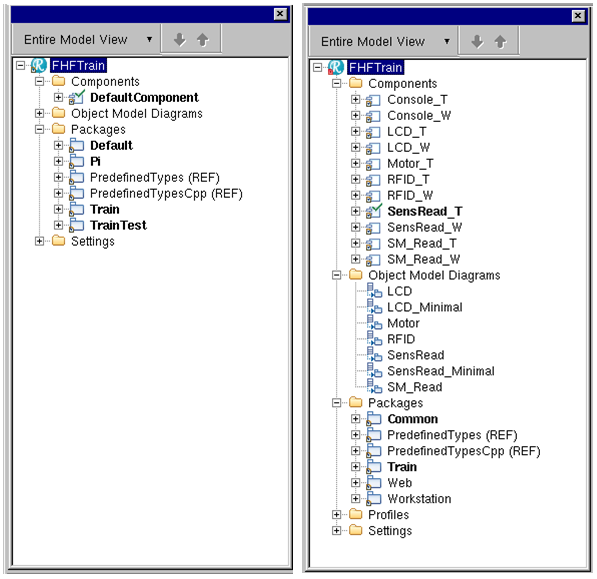
\includegraphics[width=1\textwidth]{content/pictures/train/structure.png}
	\label{pic:train_structure}
\end{figure}
Das FHFTrain-Projekt basiert auf dem Semesterprojekt des Sommersemesters 2016. Der Code, der den Zug grundsätzlich zum Fahren bringt und die Hardware ansteuert, muss also zusammen mit dem neuen Code, also Algorithmus und Socket, "gemerged" werden. In Abbildung \ref{pic:train_structure} sieht man zunächst den jeweils grundgelegenen Aufbau der beiden Projekte.\\  
Das alte Semesterprojekt beinhaltet mehrere Components, die jeweils mit T oder W beschriftet sind, für Train und Workstation.\\
Das aktuelle Projekt beinhaltet nur eine Component und mehreren Packages, jeweils für den Raspberry Pi (Als Pi bezeichnet) und den Zug (Als Train bezeichnet). Zusätzlich gibt es noch ein Testpackage, TrainTest.\\
Zunächst wird das alte Projekt geöffnet, über \textit{File->Insert Project->Existing…} lässt sich ein zweites Projekt in die Modelübersicht aufnehmen. Danach können sowohl Components, als auch Diagramme und Packages per \textit{Ctrl+Drag} übertragen werden. In der finalen Version wird die "DefaultComponent" aus dem aktuellen Projekt in die Components "Algorithm\_Socket" und "Train\_Socket" aufgeteilt. "Algorithm\_Socket" verwaltet dabei den kompletten Algorithmus und die Socket-Verbindung auf dem Pi. "Train\_Socket" hingegen ist für die Kommunikation auf dem Zug zuständig, diese Component verwaltet also, was an den Pi geschickt wird und wie die Informationen gehandhabt werden sollen, die vom Pi ankommen.\\
In Abbildung \ref{pic:train_structure_merged} ist die vollständige Modellübersicht des gemergten Projektes zu sehen.
\begin{figure}
	\caption{Aufbau des Projektes nach dem Merge}
	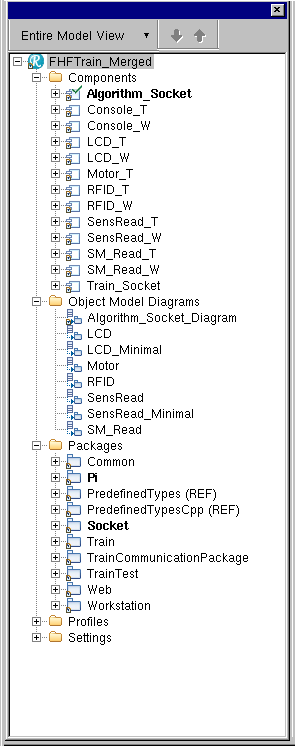
\includegraphics[height=0.8\textheight]{content/pictures/train/structure_merged.png}
	\label{pic:train_structure_merged}
\end{figure}

\section{Zusammenführung des Codes}

Nachdem beide Projekte „gemerged“ worden sind, müssen noch mehrere Stellen im Code modifiziert werden.\\
Im ersten Schritt wird eine Verbindung zwischen der Train-Kommunikation und der Shared-Memory aufgebaut. Die Shared-Memory steht allen Komponenten des Zuges zur Verfügung, über diese können die Komponenten Daten austauschen. In der Shared-Memory werden Datentypen für AfterSpeed und BeforeSpeed erstellt, also die Geschwindigkeiten, die der Zug bis zu einem Tag und ab einem Tag fahren soll.\\
Als nächstes wird eine Methode implementiert, die die Befehle des Pis in Substrings unterteilen und die Geschwindigkeiten in die Shared-Memory eintragen. Die Motor-Komponente sorgt dann automatisch dafür, dass die neue Geschwindigkeit gefahren wird.\\
Im letzten Schritt muss noch dafür gesorgt werden, dass der Zug dem Pi auch seine Position mitteilen kann. Dazu wird eine Funktion implementiert, die immer, wenn der Zug einen RFID Tag erkennt, einen dazugehörigen float-Wert in die Shared-Memory speichert. Schließlich wird noch implementiert, dass der TrainSpeaker genau dann seine Position an den Pi sendet, wenn in der Shared-Memory eine Änderung des RFID-Tags stattgefunden hat.\\
Nach diesen Arbeitsschritten sind die beiden Projekte endgültig  zu einem Projekt „gemerged“, welches dann auch funktionstüchtig ist.

\chapter{Socket}
\chapter{Tests}

% Beispielkapitel
\chapter{Einleitung}

\section{Strukturen}

\subsection{asdasd}
asdfasdf

\subsubsection{Subsubsection}
asdf

\paragraph{Paragraph}
asdf

\section{Beispielabbildungen}

\lipsum[10]

\begin{wrapfigure}{rt}{8cm}
\caption{Bildüberschrift}
\centering

\includegraphics[width=0.3\textwidth]{content/pictures/hfu}
Quelle: \cite{s11wasml}
\label{pic:bild2}
\end{wrapfigure}

\lipsum[10]

\begin{figure}
\caption{Bildüberschrift}

\includegraphics[width=1\textwidth]{content/pictures/hfu}
Quelle: \cite{s11wasml}
\label{pic:bild1}
\end{figure}

\section{Beispieltabelle}

\begin{table}
\caption{Tabellenüberschrift}
\center
\footnotesize
\begin{tabular}{lll}
\toprule
Head1 & Head2 & Head3 \\
\midrule
Val1 & Val2 & Val3 \\
Val4 & Val5 & Val6 \\
\bottomrule
\end{tabular}
\end{table}

\section{Listings}

\begin{lstlisting}[language=java, caption=Hallo Welt in Java]
public class HalloWelt 
{
	public static void main(String[] args) 
	{
		System.out.println("Hallo Welt!");
	}
}
\end{lstlisting}

\section{Abkürzungen}

Im Abkürzungsverzeichnis stehende Abkürzungen können in Langform (\ac{HFU}) oder in Kurzform (\acs{HFU}) angegeben werden.

\section{Abgesetztes wörtliches Zitat}

\lipsum[10]

\begin{quote}
\textit{\enquote{Eingerücktes wörtliches Zitat.}}\cite[S. 14ff]{s11wasml}
\end{quote}

\lipsum[10]

\section{Theoreme}

\lipsum[2]

\begin{beispiel}
Beispieltext\dots
\end{beispiel}
 
\lipsum[2]

\begin{these}
These\dots
\end{these}
 
\lipsum[2]
 
\begin{definition}
Unter dem Begriff \dots verstehen wir \dots
\end{definition}

\lipsum[2]
\chapter{Grundlagen}
\begin{figure}
\caption{Bildüberschrift}

\includegraphics[width=1\textwidth]{content/pictures/hfu}
\label{pic:bild3}
\end{figure}
\chapter{[Eigene Kapitel]}
\chapter{Ausblick}
\chapter{Fazit}

% Schalgwortverzeichnis (Index)
%\printindex

% Literaturverzeichnis
\singlespacing
\bibliographystyle{alphadin}
\bibliography{bibtex}

% Eidesstattliche Erklärung
\chapter*{Eidesstattliche Erklärung\markboth{Eidesstattliche Erklärung}{}}
% Eintrag in das Inhaltsverzeichnis 
\addcontentsline{toc}{chapter}{Eidesstattliche Erklärung}

Ich versichere, dass ich die vorstehende Arbeit selbständig verfasst und hierzu
keine anderen als die angegebenen Hilfsmittel verwendet habe. Alle Stellen der Arbeit die 
wörtlich oder sinngemäß aus fremden Quellen entnommen wurden, sind als solche kenntlich gemacht.
\\
\\
Die Arbeit wurde bisher in gleicher oder ähnlicher Form in keinem anderen
Studiengang als Prüfungsleistung vorgelegt oder an anderer Stelle
veröffentlicht.
\\
\\
Ich bin mir bewusst, dass eine falsche Erklärung rechtliche Folgen haben kann.

\vspace*{1.5cm} \par
\line(1,0){200} \par
\docOrt, den  \docAbgabedatum ~~\docVorname~\docNachname

\appendix
% Hier können Anhaenge angefuegt werden

\end{document}      